\documentclass{article}

\usepackage{tikz} 
\usetikzlibrary{automata, positioning, arrows} 

\usepackage{amsthm}
\usepackage{amsfonts}
\usepackage{amsmath}
\usepackage{amssymb}
\usepackage{fullpage}
\usepackage{color}
\usepackage{parskip}
\usepackage{hyperref}
\usepackage{float}
\usepackage[section]{placeins}
  \hypersetup{
    colorlinks = true,
    urlcolor = blue,
    linkcolor= blue,
    citecolor= blue,
    filecolor= blue,
    }
    
\usepackage{listings}
\usepackage[utf8]{inputenc}                                                    
\usepackage[T1]{fontenc}                                                       

\definecolor{dkgreen}{rgb}{0,0.6,0}
\definecolor{gray}{rgb}{0.5,0.5,0.5}
\definecolor{mauve}{rgb}{0.58,0,0.82}

\lstset{frame=tb,
  language=haskell,
  aboveskip=3mm,
  belowskip=3mm,
  showstringspaces=false,
  columns=flexible,
  basicstyle={\small\ttfamily},
  numbers=none,
  numberstyle=\tiny\color{gray},
  keywordstyle=\color{blue},
  commentstyle=\color{dkgreen},
  stringstyle=\color{mauve},
  breaklines=true,
  breakatwhitespace=true,
  tabsize=3
}

\newtheoremstyle{theorem}
  {\topsep}   % ABOVESPACE
  {\topsep}   % BELOWSPACE
  {\itshape\/}  % BODYFONT
  {0pt}       % INDENT
  {\bfseries} % HEADFONT
  {.}         % HEADPUNCT
  {5pt plus 1pt minus 1pt} % HEADSPACE
  {}
\theoremstyle{theorem} 
   \newtheorem{theorem}{Theorem}[section]
   \newtheorem{corollary}[theorem]{Corollary}
   \newtheorem{lemma}[theorem]{Lemma}
   \newtheorem{proposition}[theorem]{Proposition}
\theoremstyle{definition}
   \newtheorem{definition}[theorem]{Definition}
   \newtheorem{example}[theorem]{Example}
\theoremstyle{remark}    
  \newtheorem{remark}[theorem]{Remark}

\title{CPSC-354 Report}
\author{Ethan Tapia  \\ Chapman University}

\date{\today} 

\begin{document}

\maketitle

\begin{abstract}
\end{abstract}

\setcounter{tocdepth}{3}
\tableofcontents

\section{Introduction}\label{intro}

\section{Week by Week}\label{homework}

% =========================
% Week 1 
% =========================
\subsection{Week 1}

\textbf{Lecture Summary}

We introduced \emph{formal systems} and worked with Hofstadter’s MIU-system as a rule–based rewriting game.  
Alphabet: $\Sigma=\{M,I,U\}$.  
Axiom (start string): $MI$.  
Production rules:
\begin{enumerate}
    \item[\textbf{(R1)}] If a string ends in $I$, append $U$: $xI \Rightarrow xIU$.
    \item[\textbf{(R2)}] If a string is $Mx$, duplicate $x$: $Mx \Rightarrow Mxx$.
    \item[\textbf{(R3)}] Replace any $III$ by $U$: $xIIIy \Rightarrow xUy$.
    \item[\textbf{(R4)}] Delete any $UU$: $xUUy \Rightarrow xy$.
\end{enumerate}
Key idea: reason about \emph{invariants} that rules preserve, instead of searching blindly through derivations.

\bigskip
\textbf{Homework: The MU-puzzle}

\begin{definition}[I–count and residue]
For a string $w$, let $\#_I(w)$ be the number of $I$’s in $w$, and define the residue
\[
\varphi(w) \;=\; \#_I(w) \bmod 3 \in \{0,1,2\}.
\]
\end{definition}

\begin{lemma}[Effect of each rule on $\#_I$]\label{lem:rule-effects}
For any string $w$:
\begin{enumerate}
    \item \textbf{(R1)} and \textbf{(R4)} do not change $\#_I$.
    \item \textbf{(R2)} doubles the number of $I$’s \emph{after} the initial $M$, so $\varphi$ is multiplied by $2$ modulo $3$.
    \item \textbf{(R3)} decreases $\#_I$ by $3$, so $\varphi$ is unchanged.
\end{enumerate}
\end{lemma}

\begin{proposition}[Invariant modulo $3$]\label{prop:invariant}
Every string derivable from $MI$ has $\varphi\in\{1,2\}$. In particular, no derivable string has $\varphi=0$.
\end{proposition}

\begin{proof}
We use induction on the length of a derivation from $MI$.

\emph{Base.} $\varphi(MI)=1$.

\emph{Step.} Assume $\varphi\in\{1,2\}$ for some derivable $w$.  
By Lemma~\ref{lem:rule-effects}, rules (R1), (R3), and (R4) keep $\varphi$ unchanged, and rule (R2) maps $1\leftrightarrow 2$ modulo $3$. None of these operations yields $0$ from a value in $\{1,2\}$. Therefore the next string also has $\varphi\in\{1,2\}$.
\end{proof}

\begin{theorem}[MU is unreachable]
\label{thm:mu-unreachable}
$MU$ cannot be derived from $MI$ in the MIU-system.
\end{theorem}

\begin{proof}
$MU$ contains zero $I$’s, hence $\varphi(MU)=0$. By Proposition~\ref{prop:invariant}, every derivable string has residue $1$ or $2$. Thus $MU$ is not derivable.
\end{proof}

\textit{Conclusion.} Starting from $MI$ we can toggle the residue $1\leftrightarrow 2$ with (R2) and otherwise keep it fixed with (R1), (R3), (R4). We never reach residue $0$, so no sequence of legal rule applications yields $MU$.

\begin{center}
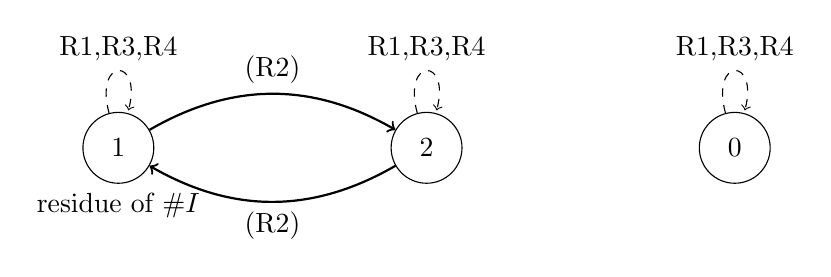
\begin{tikzpicture}[node distance=3cm, auto]
  \tikzstyle{state}=[circle,draw,minimum size=9mm]
  \node[state, label=below:{residue of $\#I$}] (Z1) {1};
  \node[state, right=of Z1] (Z2) {2};
  \node[state, right=of Z2] (Z0) {0};
  \path[->, thick]
    (Z1) edge[bend left] node[above]{(R2)} (Z2)
    (Z2) edge[bend left] node[below]{(R2)} (Z1);
  \path[->, dashed]
    (Z1) edge[loop above] node{R1,R3,R4} ()
    (Z2) edge[loop above] node{R1,R3,R4} ()
    (Z0) edge[loop above] node{R1,R3,R4} ();

\end{tikzpicture}
\end{center}
\textbf{Question:} If the MU-puzzle shows that some goals are unreachable due to invariants (like the mod-3 property of I’s), how does this idea connect to undecidability in programming languages?

\FloatBarrier

% =========================
% Week 2 
% =========================
\subsection{Week 2}

\textbf{Lecture Summary} \\
We introduced \emph{Abstract Reduction Systems (ARS)}: a pair $(A,R)$ with one-step reduction $R\subseteq A\times A$. Key notions:
reducible/normal form, joinability, confluence, termination, and unique normal forms.

\bigskip
\textbf{Homework Part 2: The 8 Combinations}

We provide an example ARS for each combination of
$(\text{confluent}, \text{terminating}, \text{unique NFs})$.
If a row is impossible, we explain why.

\begin{center}
\begin{tabular}{|c|c|c|l|}
\hline
\textbf{Confluent} & \textbf{Terminating} & \textbf{Unique NFs} & \textbf{Example} \\
\hline
True  & True  & True  & $A=\{a\},\ R=\emptyset$ (Fig.~\ref{fig:combo-ttt}) \\
True  & True  & False & \emph{Impossible} \\
True  & False & True  & $A=\{a,b\},\ R=\{(a,a),(a,b)\}$ (Fig.~\ref{fig:combo-tft}) \\
True  & False & False & $A=\{a\},\ R=\{(a,a)\}$ (Fig.~\ref{fig:combo-tff}) \\
False & True  & True  & \emph{Impossible} \\
False & True  & False & $A=\{a,b,c\},\ R=\{(a,b),(a,c)\}$ (Fig.~\ref{fig:combo-ftf}) \\
False & False & True  & \emph{Impossible} \\
False & False & False & $A=\{a,b,c\},\ R=\{(a,b),(a,c),(b,b),(c,c)\}$ (Fig.~\ref{fig:combo-fff}) \\
\hline
\end{tabular}
\end{center}

\noindent\textit{Why some rows are impossible.}
If an ARS has unique normal forms, it must be confluent.
If an ARS is both confluent and terminating, then every element reduces to a unique normal form.
Therefore the rows \((\text{T},\text{T},\text{F})\), \((\text{F},\text{T},\text{T})\), and \((\text{F},\text{F},\text{T})\) cannot occur.

\begin{figure}[H]
\centering
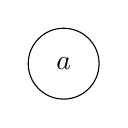
\begin{tikzpicture}[->,>=stealth',node distance=3cm,auto]
  \tikzstyle{obj}=[circle,draw,minimum size=9mm]
  \node[obj] (a) {$a$};
\end{tikzpicture}
\caption{Combination (True, True, True). Terminating, confluent, unique NF.}
\label{fig:combo-ttt}
\end{figure}

\begin{figure}[H]
\centering
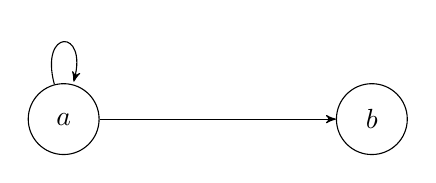
\begin{tikzpicture}[->,>=stealth',node distance=3cm,auto]
  \tikzstyle{obj}=[circle,draw,minimum size=9mm]
  \node[obj] (a) {$a$};
  \node[obj] (b) [right=of a] {$b$};
  \path (a) edge (b)
        (a) edge[loop above] (a);
\end{tikzpicture}
\caption{Combination (True, False, True). Non-terminating, confluent, unique NF $b$.}
\label{fig:combo-tft}
\end{figure}

\begin{figure}[H]
\centering
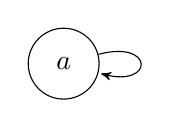
\begin{tikzpicture}[->,>=stealth',node distance=3cm,auto]
  \tikzstyle{obj}=[circle,draw,minimum size=9mm]
  \node[obj] (a) {$a$};
  \path (a) edge[loop right] (a);
\end{tikzpicture}
\caption{Combination (True, False, False). Non-terminating, confluent, no normal form.}
\label{fig:combo-tff}
\end{figure}

\begin{figure}[H]
\centering
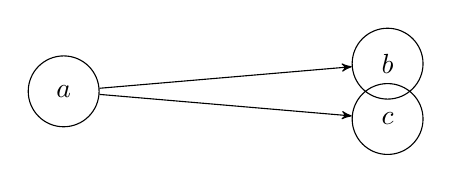
\begin{tikzpicture}[->,>=stealth',node distance=3.2cm,auto]
  \tikzstyle{obj}=[circle,draw,minimum size=9mm]
  \node[obj] (a) {$a$};
  \node[obj] (b) [right=of a,yshift=10pt] {$b$};
  \node[obj] (c) [right=of a,yshift=-10pt] {$c$};
  \path (a) edge (b)
        (a) edge (c);
\end{tikzpicture}
\caption{Combination (False, True, False). Terminating, not confluent; two distinct normal forms $b,c$ are not joinable.}
\label{fig:combo-ftf}
`\end{figure}

\begin{figure}[H]
\centering
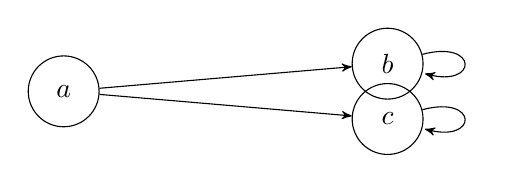
\begin{tikzpicture}[->,>=stealth',node distance=3.2cm,auto]
  \tikzstyle{obj}=[circle,draw,minimum size=9mm]
  \node[obj] (a) {$a$};
  \node[obj] (b) [right=of a,yshift=10pt] {$b$};
  \node[obj] (c) [right=of a,yshift=-10pt] {$c$};
  \path (a) edge (b)
        (a) edge (c)
        (b) edge[loop right] (b)
        (c) edge[loop right] (c);
\end{tikzpicture}
\caption{Combination (False, False, False). Non-terminating (loops), not confluent, no unique normal forms.}
\label{fig:combo-fff}
\end{figure}

\FloatBarrier

\noindent\paragraph{Conclusion.}
The MU-puzzle illustrates how invariants prove impossibility in a formal system.
The ARS framework provides the general language to study rewrite systems via termination, confluence, and normal forms.
The 8-combination analysis shows which behaviors are possible and which are structurally impossible.

\noindent\paragraph{Question:}
Could there be a general framework that unifies invariants with confluence and termination, so that impossibility and determinism appear as two sides of the same rewriting theory?

\subsection{Week 3}
\textbf{Lecture Summary}
\\TBD

\textbf{Homework 3}
\paragraph{Exercise 5}

Consider an ARS with
[
A = {a,b}^* = {\varepsilon, a, b, aa, ab, ba, bb, aaa, \dots },
]
and rewrite rules
[
ab \to ba, \qquad 
ba \to ab, \qquad 
aa \to \varepsilon, \qquad 
b \to \varepsilon.
]

\begin{enumerate}
   \textbf{Reduce some example strings such as $abba$ and $bababa$.}
  \begin{align}
    abba &\to aa \to \varepsilon, \
    bababa &\to aaa \to a.
  \end{align}

   \textbf{Find two strings that are not equivalent. How many non-equivalent strings can you find?}
  \begin{itemize}
    \item $\varepsilon$
    \item $a$
  \end{itemize}
  These have different normal forms and cannot be transformed into each other.

   \textbf{How many equivalence classes does $\stackrel{\ast}{\longleftrightarrow}$ have? What are the normal forms?} \
  There are two equivalence classes:
  \begin{enumerate}
    \item Strings whose normal form is $\varepsilon$,
    \item Strings whose normal form is $a$.
  \end{enumerate}
  The class is determined by the parity of the number of $a$’s in the string.

   \textbf{Can you modify the ARS so that it becomes terminating without changing its equivalence classes?} \
  Yes. Remove one of the first two rules. They only permute $a$ and $b$ and do not affect equivalence classes, but having both makes the system non-terminating.

   \textbf{Question.} \
If I remove all the $b$’s from a string, does the remaining word reduce to $a$ or to $\varepsilon$?”  
\ans\ This can be answered using the ARS because $b \to \varepsilon$ always deletes $b$’s, and the final result depends only on whether the number of $a$’s left is odd or even. Odd $\mapsto a$, even $\mapsto \varepsilon$.

\end{enumerate}
\paragraph{Exercise 5b}

Now replace the rule $aa \to \varepsilon$ with $aa \to a$.

\begin{enumerate}
  \item \textbf{Reduce some example strings such as $abba$ and $bababa$.}
  \begin{align}
    abba &\to aa \to a, \
    bababa &\to aaa \to aa \to a.
  \end{align}

  \item \textbf{Find two strings that are not equivalent.}
  \begin{itemize}
    \item $\varepsilon$
    \item $a$
  \end{itemize}

   \textbf{How many equivalence classes are there? What are the normal forms?} \
  There are two equivalence classes:
  \begin{enumerate}
    \item Strings with no $a$’s $;\to;$ normal form $\varepsilon$,
    \item Strings with at least one $a$ $;\to;$ normal form $a$.
  \end{enumerate}

 \textbf{Modify the ARS to make it terminating.} \
  As above, remove one of the two swapping rules $ab \leftrightarrow ba$.

   \textbf{Question:} \
  Is the system confluent? That is, if a string can be reduced in two different ways, do the reductions always lead to the same normal form?

\end{enumerate}


\section{Evidence of Participation}

\section{Conclusion}\label{conclusion}

\begin{thebibliography}{99}
\bibitem[BLA]{bla} Author, \href{https://en.wikipedia.org/wiki/LaTeX}{Title}, Publisher, Year.
\end{thebibliography}

\end{document}
